\documentclass[10pt]{beamer}
\usetheme[
%%% options passed to the outer theme
%    progressstyle=movCircCnt,   %either fixedCircCnt, movCircCnt, or corner
%    rotationcw,          % change the rotation direction from counter-clockwise to clockwise
%    shownavsym          % show the navigation symbols
  ]{AAUsimple}
  
% If you want to change the colors of the various elements in the theme, edit and uncomment the following lines
% Change the bar and sidebar colors:
%\setbeamercolor{AAUsimple}{fg=red!20,bg=red}
%\setbeamercolor{sidebar}{bg=red!20}
% Change the color of the structural elements:
%\setbeamercolor{structure}{fg=red}
% Change the frame title text color:
%\setbeamercolor{frametitle}{fg=blue}
% Change the normal text color background:
%\setbeamercolor{normal text}{fg=black,bg=gray!10}
% ... and you can of course change a lot more - see the beamer user manual.

\usepackage[utf8]{inputenc}
\usepackage[english]{babel}
\usepackage[T1]{fontenc}
% Or whatever. Note that the encoding and the font should match. If T1
% does not look nice, try deleting the line with the fontenc.
\usepackage{helvet}

% colored hyperlinks
\newcommand{\chref}[2]{%
  \href{#1}{{\usebeamercolor[bg]{AAUsimple}#2}}%
}

\title{Smart meter security: a survey by Ross Anderson}

\subtitle{Specialization Course in Distributed Systems}  % could also be a conference name

\date{\today}

\author{
  Bruno Thalmann\\
  \href{mailto:bthalm11@student.aau.dk}{{\tt bthalm11@student.aau.dk}}
}

% - Give the names in the same order as they appear in the paper.
% - Use the \inst{?} command only if the authors have different
%   affiliation. See the beamer manual for an example

\institute[
%  {\includegraphics[scale=0.2]{aau_segl}}\\ %insert a company, department or university logo
  Dept.\ of Computer Science\\
  Aalborg University\\
  Denmark
] % optional - is placed in the bottom of the sidebar on every slide
{% is placed on the bottom of the title page
  Department of Computer Science\\
  Aalborg University\\
  Denmark
  
  %there must be an empty line above this line - otherwise some unwanted space is added between the university and the country (I do not know why;( )
}

% specify a logo on the titlepage (you can specify additional logos an include them in 
% institute command below
\pgfdeclareimage[height=1.5cm]{titlepagelogo}{AAUgraphics/aau_logo_new} % placed on the title page
%\pgfdeclareimage[height=1.5cm]{titlepagelogo2}{AAUgraphics/aau_logo_new} % placed on the title page
\titlegraphic{% is placed on the bottom of the title page
  \pgfuseimage{titlepagelogo}
%  \hspace{1cm}\pgfuseimage{titlepagelogo2}
}

\begin{document}
% the titlepage
{\aauwavesbg%
\begin{frame}[plain,noframenumbering] % the plain option removes the header from the title page
  \titlepage
\end{frame}}
%%%%%%%%%%%%%%%%

% TOC
\begin{frame}{Agenda}{}
\tableofcontents
\end{frame}
%%%%%%%%%%%%%%%%

\section{Introduction}
% motivation for creating this theme
\begin{frame}{Introduction}{}
	\begin{itemize}
		\item Overview
		
		\hfil
		\item Context
		
		\hfil
		\item Examples
	\end{itemize}
\end{frame}
%%%%%%%%%%%%%%%%

\subsection{Smart Meter}
\begin{frame}{Smart Meter}
\begin{itemize}
\item A device that records electricity, gas or water consumption in a household
\\~\\
\begin{center}
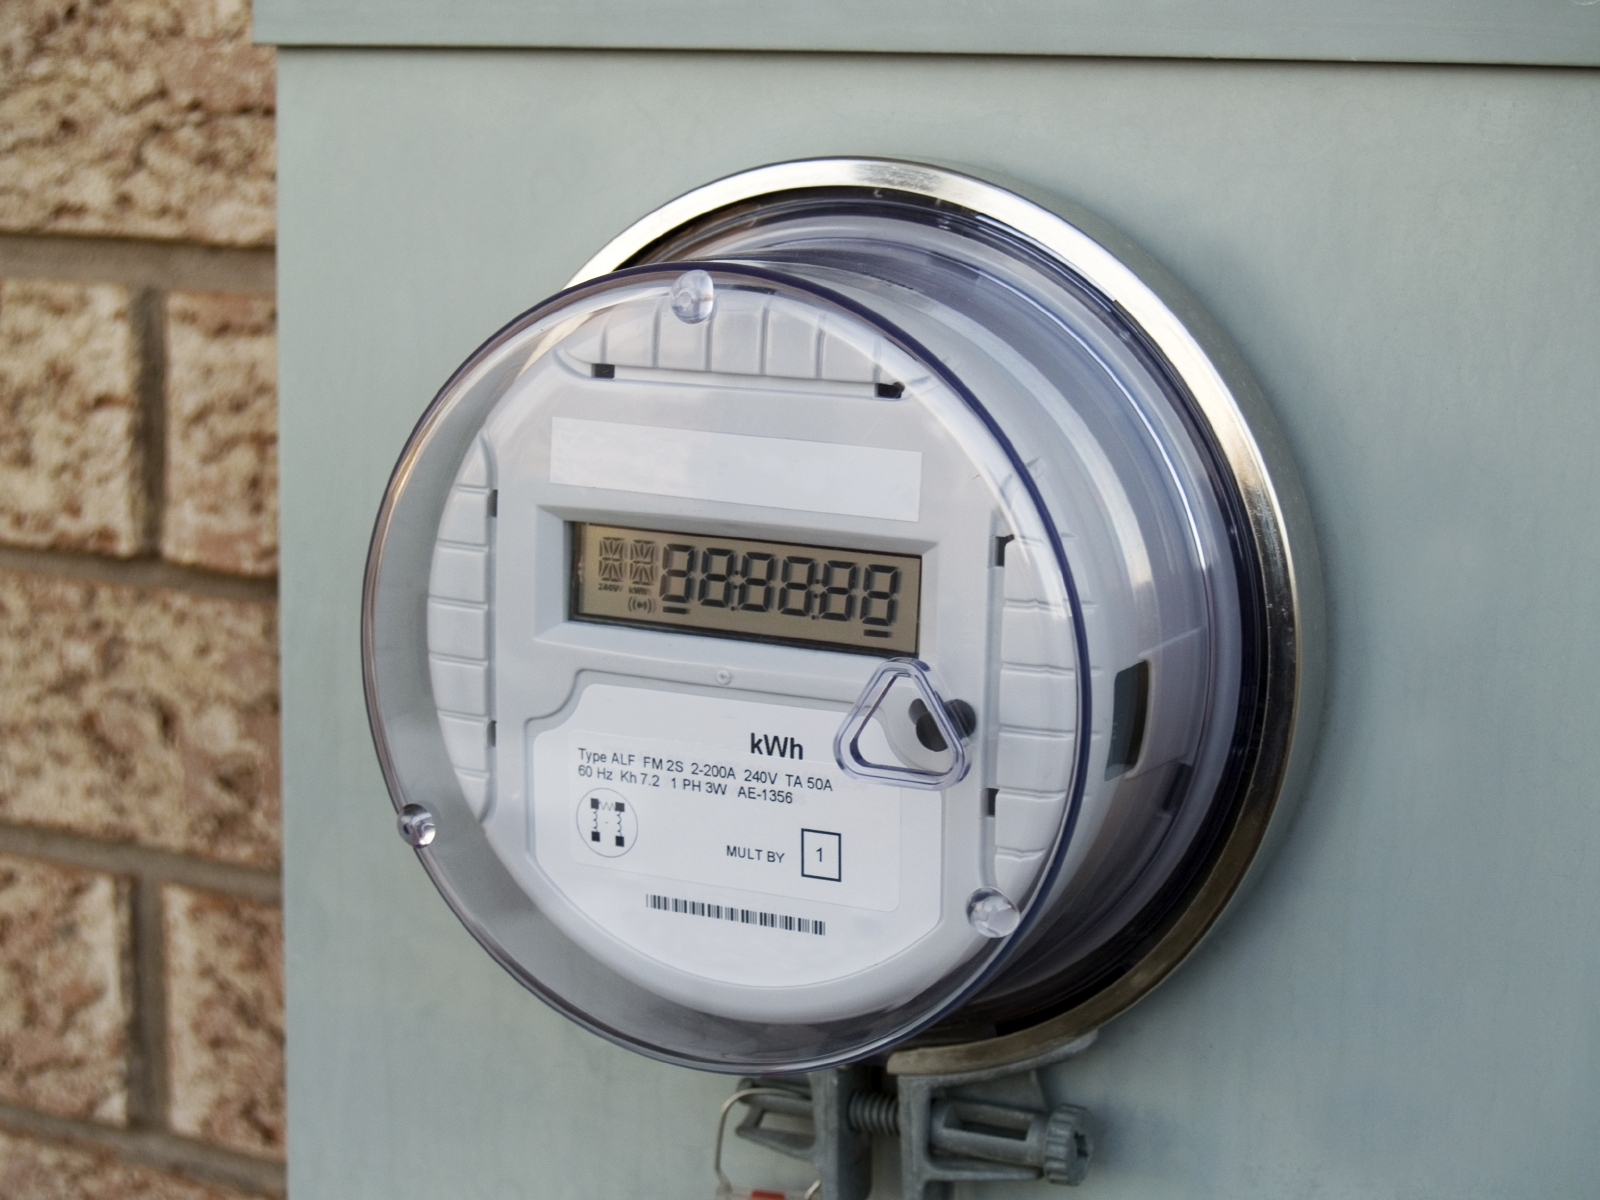
\includegraphics[scale=.25]{./graphics/smart_meter}
\end{center}
\end{itemize}
\end{frame}

\section{Prepayment}
\subsection{Prepayment}
\begin{frame}{South African Example}{Prepayment}
  \begin{itemize}
  	\item Why prepayment?
  	\begin{itemize}
  		\item Poor households
  		\item Informal accommodation
  	\end{itemize}
    \item Parties
    \begin{itemize}
    	\item Eskom - state owned
    	\item Local electricity distributors
    	\item Token vending agents
    	\item Customers vendors
    	\item Equipment vendors
    \end{itemize}
    \item Issues
    \begin{itemize}
    	\item Brownout
    	\item Token vending machines
    \end{itemize}
  \end{itemize}
\end{frame}
%%%%%%%%%%%%%%%%

\section{Security Economics}
\begin{frame}{South African Example}{Security Economics}
	\begin{itemize}
		\item Going from credit to prepayment resulted in 10\% reduced energy usage
		\item Same in Northern Ireland, Russia and Brazil
		\item People care more about their usage because they have to go to the vending station and use their ATM card or cash
		\item Easy debt management - no court order, no replacement of meter 
	\end{itemize}
\end{frame}

\subsection{Smart Meter Fraud}
\begin{frame}{Smart Meter Fraud}{General}
	\begin{itemize}
		\item Vulnerabilities will get industrialised
		\item The South African example shows this 
		\item Fixing a bug is very expensive
		\item Replacing 100 million meters in Europe would take 5 years and cost \$20bn
	\end{itemize}
\end{frame}
%%%%%%%%%%%%%%%%

\section{Privacy}
\begin{frame}{Smart Meter Data}{Privacy issues}
	\begin{itemize}
		\item Smart meter data in Europe is recorded in fine granularity
		\\~\\
		\item Extract personal information by analysing the meter data
		\begin{itemize}
			\item How many live in the house?
			
			\item When are they asleep?
			\item Are they home at the moment?
		\\~\\	
		\end{itemize}
		\item Home appliance vendors, burglars etc.
		\\~\\
		\item Customer vs energy company owned data
	\end{itemize}
\end{frame}
%%%%%%%%%%%%%%%%


\begin{frame}{Smart Meter Data}{Who owns it?}
	\begin{itemize}
		\item Most countries move toward customer owned data
		\\~\\
		\item The tussle is the granularity one should share
		\\~\\
		\item Energy company: 48 readings per 24h
		\\~\\
		\item Customer: Only enough for billing
		\\~\\
		\item European Convention on Human Rights: European citizens have the right to respect for the privacy	of their family life.
	\end{itemize}
\end{frame}
%%%%%%%%%%%%%%%%

\section{Architecture}
\subsection{Differences in Europe}
\begin{frame}{Differences in Europe}
	\begin{itemize}
	\item Italy - monopoly
		\item Germany - a customer can choose an energy company
		\begin{itemize}
			\item Company sets up smart meter
			\item Disliked because fewer smart meters were sold
		\end{itemize}
		\item United Kingdom - centralised system by a Data Communication Company
			\begin{itemize}
				\item Same smart meter
				\item Easy switch of energy company
				\item Wash now or later - privacy, smart meter support
			\end{itemize}
			
			                      	\item When the wind blows in Germany
			                      	\item There needs to be some sort of communication between the market and the smart meter
	\end{itemize}
\end{frame}



\subsection{Strategic Vulnerabilities}
\begin{frame}{Centralised Metering System}{Pros and cons}
\begin{itemize}
	\item Used in the UK
	\\~\\
	\item Avoid rolling out a truck to the customer
	\\~\\
	\item When countries are in conflict - energy is a target
	\\~\\
	\item Remote computer exploits, vulnerabilities:
	\begin{itemize}
		\item Software upgrade
		\item Tariff setting
		\item Billing
		\item API attacks
		\item Applets
	\end{itemize}
	~\\
	\item General problem: Replacing hardware is expensive
\end{itemize}
\end{frame}
%%%%%%%%%%%%%%%%z


\subsection{Opportunities}
\begin{frame}{Oppurtunities}
	\begin{itemize}
		\item Air-condition example
		\\~\\
		\item Customer web-interface
		\\~\\
		\item Control the data granularity and when devices are used
	\end{itemize}
\end{frame}

\section{Possible Solution}
\begin{frame}
	\begin{itemize}
		\item Open Home Controller
		\item Apache server - A way for the customer to manage appliances
		\item The situation right now:
	\end{itemize}
	~\\
	\begin{center}
	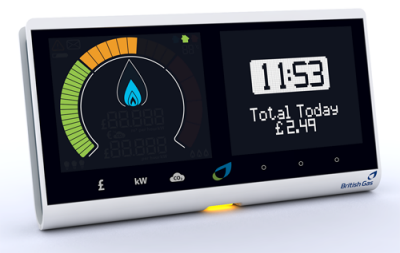
\includegraphics[scale=.25]{./graphics/smart_meter_display}
	\end{center}
\end{frame}

{\aauwavesbg
\begin{frame}[plain,noframenumbering]
  \finalpage{Questions}
\end{frame}}
%%%%%%%%%%%%%%%%

\end{document}
